\chapter{The Central Limit Theorem in Action}

\setcounter{problem}{1}

\section{Discussion}

\begin{fullwidth}

The goal of this lab is to observe how the sample means of uniform and exponential random variables have normal distributions with $N(\mu, \sigma^2/n)$ where $\sigma^2$ is the variance of the underlying distribution and $n$ is the sample size whose mean we compute. Use filenames {\tt clt\_unif.py}, {\tt clt\_exp.py} for this lab.

\section{Discussion}

The CLT in a nutshell says that the sample mean, $X\_$, of samples $X$ of size $n$
from lots of distributions follows the normal distribution,specifically, $N(\mu, \sigma^2/n)$ for sample size $n$.
 In this lab will use $U(0,1)$ and the exponential distribution with $\lambda=1.5$
and verify that using the mean as a random variable, the histogram shows a normal distribution of $N(0.5,1/12)$ for the uniform and $N(\lambda^{-1}, \lambda^{-2}/n)$ for the exponential distribution. The mean of the uniform distribution is $\frac{a+b}{2}$ and the variance is $\frac{(b-a)^2}{12}$. The mean of the exponential distribution is $\mu = \lambda^{-1}$ and its variance is $\sigma^2 = \lambda^{-2}/n$.

The key thing here is to note that not only is the distribution of the mean random variable normal, but its variance gets tighter as we increase the sample size. 

The law of large numbers says that the average of a large number of trials should approach the theoretical mean. That means that our sample mean:

\[
\bar X = \frac{1}{n} \sum_{i=1}^{n} x_i
\]

\noindent will converge to $\mu$ as $n$ approaches infinity with probability 1.

Also note that the number of trials we do improves the resolution of our normal distribution but doesn't change the variance.

\section{CLT applied to uniform random variables}


\subsection{Steps}

\step Import the usual libraries for plotting and then define these constants:

\begin{pyverbatim}
N = 4  # sample size (i.e, array size len(X))
TRIALS = 500 # how many samples we will take from the uniform distribution
\end{pyverbatim}

\noindent Now, we need to build a loop that gets  {\tt TRIALS} $X$ vectors of size $N$ with values from $U(0,1)$. Use your {\tt runif()} function. Compute the mean of each $X$ vector and add it to the end of a different array $X\_$.

\step Plot the histogram of {\tt X\_}:

\begin{pyverbatim}
# plot density of means (normalized histogram of means)
# WARNING: bins=40 is to show changes in resolution
#          where normally it's best to let the hist()
#          choose the bins for smoother view
plt.hist(X_, bins=40, normed=1)
\end{pyverbatim}

\step Your histogram should look like this \\

\scalebox{.35}{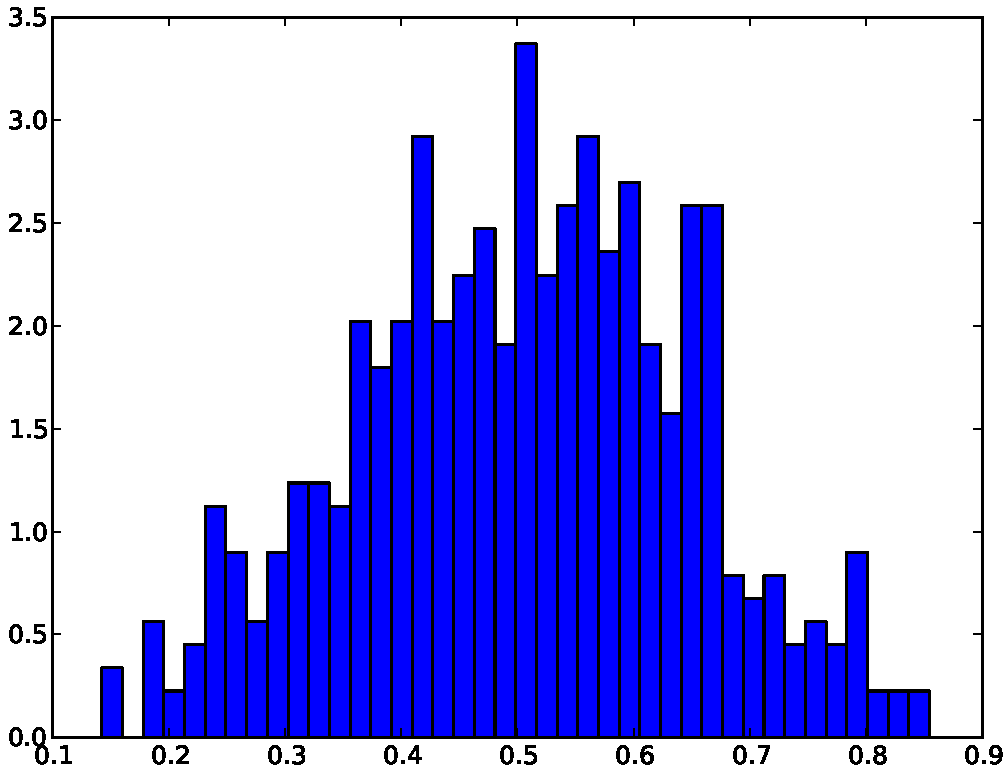
\includegraphics{figures/clt_unif-500-4-basic.pdf}}
    
Cool.  It looks kind of like a normal distribution to me. Let's add the theoretical normal distribution on top. To do that we need the appropriate parameters of $Normal(\mu, \sigma^2/n)$. The mean  $\mu$ of uniform samples should be midway between $a$ and $b$ from $U(a,b)$. In our case, that's 0.5 since we are doing $U(0,1)$. The variance of the uniform distribution is $(b-a)^2/12$ and we need the variance divided by sample size $N$.  Define a function that returns the variance of uniform distribution $U(a,b)$:

\begin{pyverbatim}
def unifvar(a, b):
    ...
\end{pyverbatim}

\step  To get the theoretical distribution, let's define it ourselves:

\begin{pyverbatim}
def normpdf(x, mu, sigma): # sigma is the standard deviation, sigma^2 is the variance
    """
    Accept either a floating-point number or a numpy ndarray, such as what you get
    from arange().  You do not need a loop in the code does not change here
    because 2 * ndarray is another ndarray automatically. In this respect,
    numpy is very convenient and behaves like R.
    """
    ...
\end{pyverbatim}

\noindent The function in math notation is:

\[
P(x) = \frac{1}{{\sigma \sqrt {2\pi } }}e^{{{ - \left( {x - \mu } \right)^2 } \mathord{\left/ {\vphantom {{ - \left( {x - \mu } \right)^2 } {2\sigma ^2 }}} \right. \kern-\nulldelimiterspace} {2\sigma ^2 }}}
\]

\step Then, plot the theoretical normal distribution on top of the histogram and set the axes so that we can use the same range throughout the next series of tests to see how the distribution changes. Note that the usual normal density function provided above expects the {\bf standard deviation not the variance} and so we need to pass {\tt normpdf()} the square root of the expected variance.

\begin{pyverbatim}
# plot real normal curve N(0.5, sigma^2/n)
x = np.arange(min(X_), max(X_), 0.01)
y = normpdf(x, 0.5, FILL THIS IN))
plt.axis([.1,.9,0,7])
plt.plot(x,y, color='red')
\end{pyverbatim}

\step Run it. The resulting graph should look like this \\

\scalebox{.35}{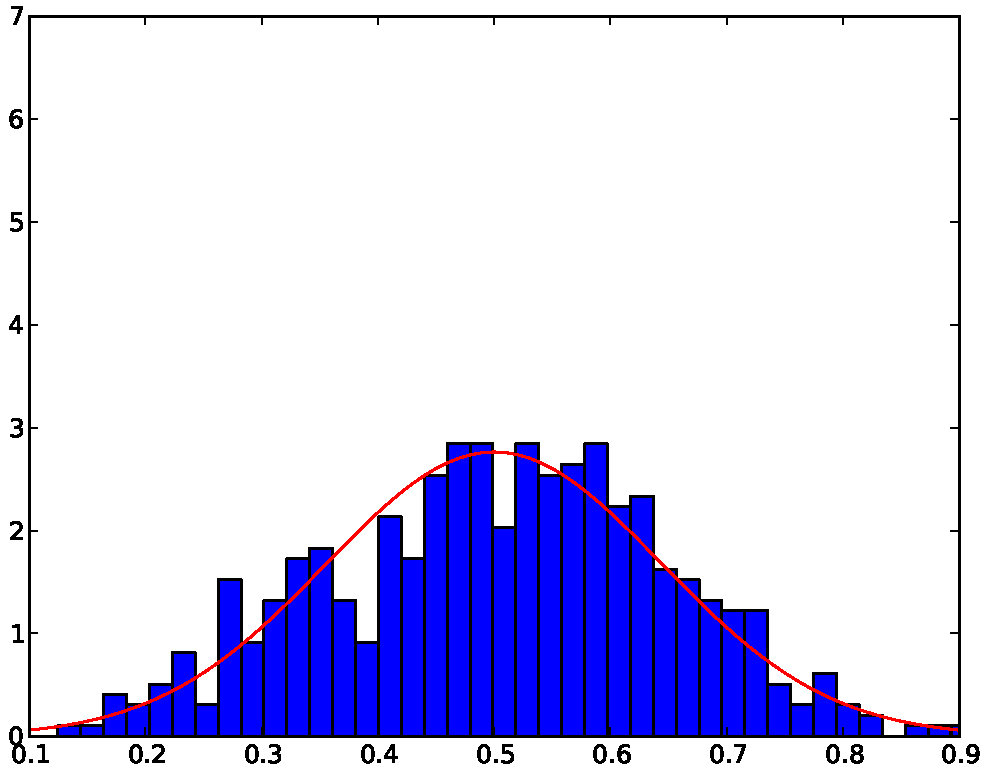
\includegraphics{figures/clt_unif-500-4-fancy.pdf}}

\step Now, display some important parameters in the graph using {\tt text()}. You will need to do that {\tt fig.add\_subplot(111)} thing again early in your script. The text in between the \$ symbols is latex and lets us display nice math symbols (e.g., the title), although I'm not doing much with it here.

{\small
\begin{pyverbatim}
plt.text(.02,.9, '$N = %d$' % N, transform = ax.transAxes)
plt.text(.02,.85,'$TRIALS = %d$' % TRIALS, transform = ax.transAxes)
plt.text(.02,.8, 'mean($\\overline{X}$) = %f' % np.mean(X_), transform = ax.transAxes)
plt.text(.02,.75,'var($\\overline{X}$) = %f' % np.var(X_), transform = ax.transAxes)
plt.text(.02,.7, 'var U($0,1$)/%d = %f' % (N,varunif(0,1)/N), transform = ax.transAxes)

plt.title("CLT Density Demo. sample mean of U(0,1) is $N(.5, \sigma^2/N)$")
plt.xlabel("$\\overline{X}$", fontsize=16)
plt.ylabel("Density", fontsize=16)
\end{pyverbatim}
}

\step Run it. The resulting graph should look like this \\

\scalebox{.35}{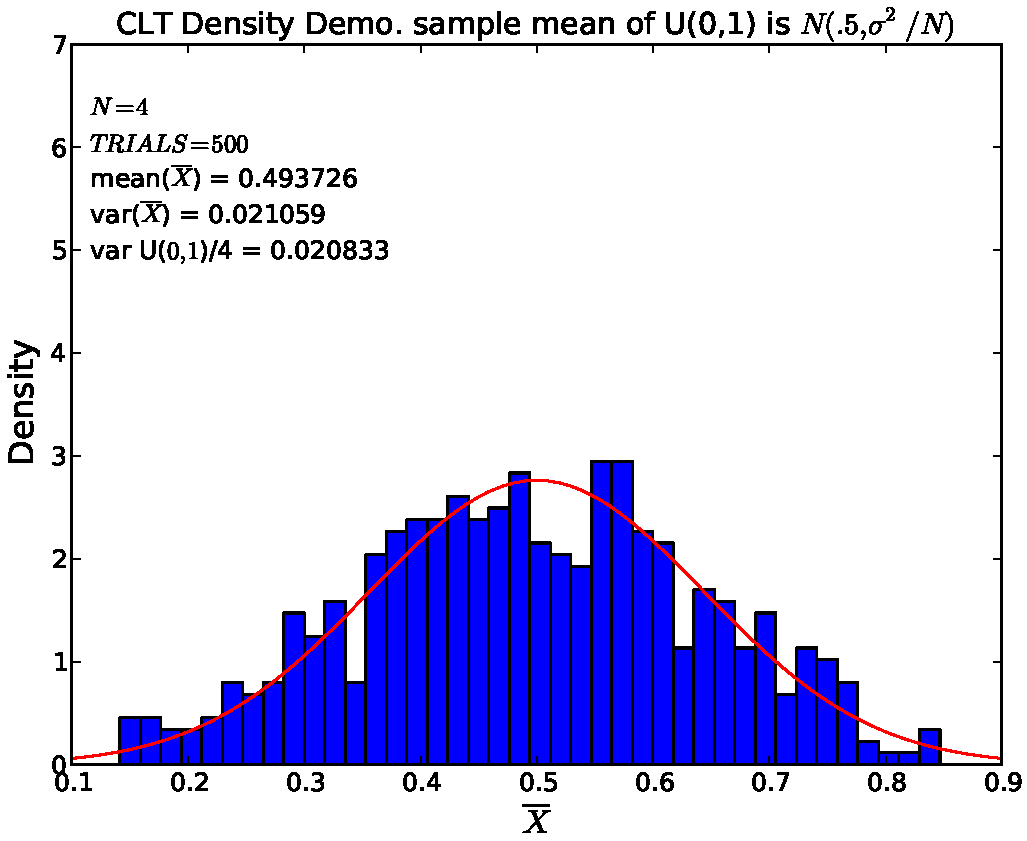
\includegraphics{figures/clt_unif-500-4-fancier.pdf}}

Notice how the mean is close to the expected 0.5 and that the variance of the sample mean is close to the theoretical variance.\\

\step Increasing the number of trials two 2000 shows much higher resolution but does not change the variance/tightness of the distribution at all. Run it and see the following:

\scalebox{.35}{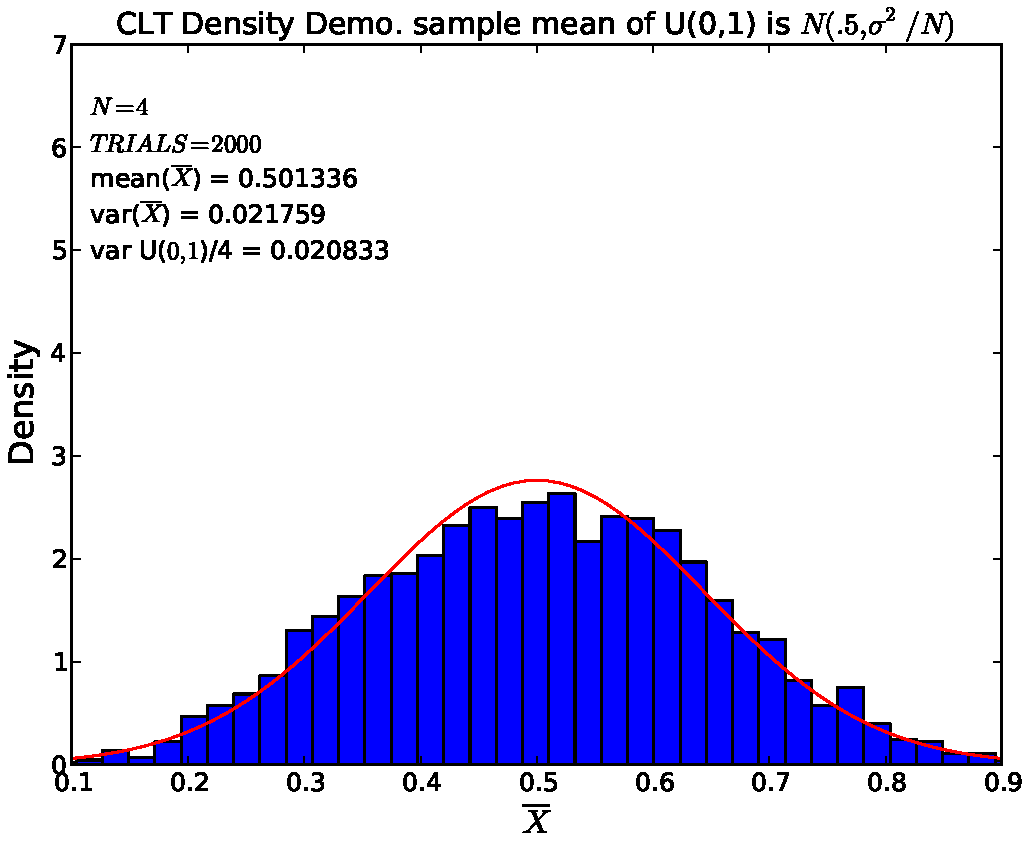
\includegraphics{figures/clt_unif-2000-4.pdf}}

\step Now, if we increase the sample size to $N=10$, we get a much tighter variance on the mean of $\overline{X}$. Run it:

\scalebox{.35}{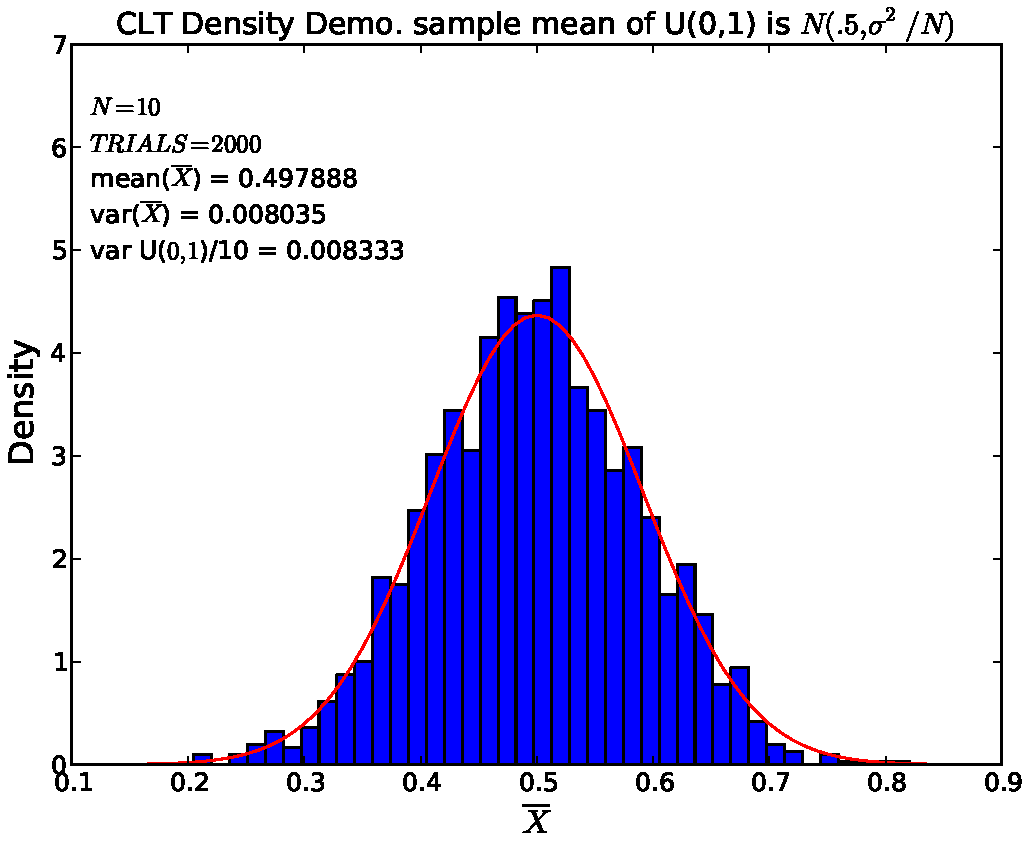
\includegraphics{figures/clt_unif-2000-10.pdf}}

\step Increasing to 20 we get:

\scalebox{.35}{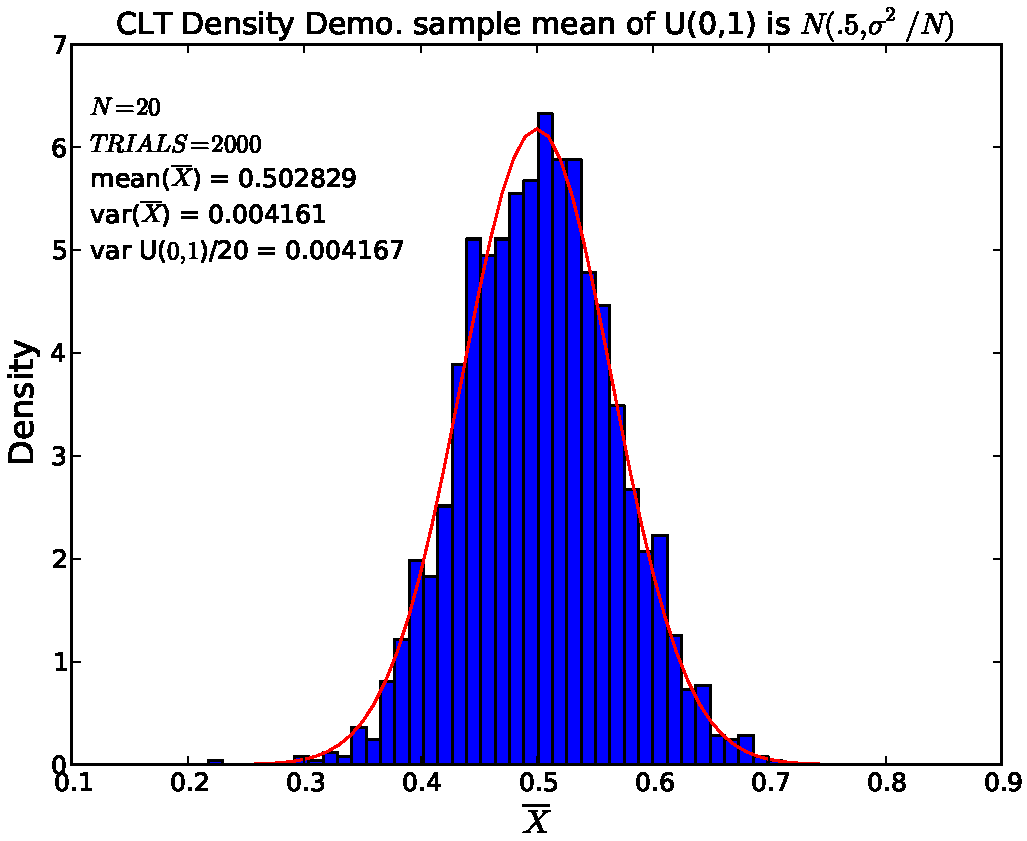
\includegraphics{figures/clt_unif-2000-20.pdf}}

\section{CLT applied to exponential random variables}

Now let's look at how the central limit theorem still gives us a normal distribution even when we pull random variables from a skewed distribution like the exponential. Create and edit a new file {\tt clt\_exp.py}.

\subsection{Steps}

\step Import the {\tt rexp(lambduh)} function you wrote for the previous lab to get exponential random variables and start out with the following constants:

\begin{pyverbatim}
N = 10
TRIALS = 4000
LAMBDUH = 1.5
\end{pyverbatim}

\step Repeat the loop we did above to get the mean of a bunch of samples into $X\_$, but this time from the exponential distribution {\tt rexp(LAMBDUH)} instead of the uniform distribution function. Plot the histogram of $X\_$ as you did before, using a bin size of 40.

\step Plot the theoretical normal distribution on top using your {\tt normpdf()} (you can cut/paste it into {\tt clt\_exp.py}). The mean of the exponential distribution is $\mu = \lambda^{-1}$ and its variance is $\sigma^2 = \lambda^{-2}$.

\begin{pyverbatim}
# plot real normal curve N(lambda^-1, sigma^-2 / N)
x = np.arange(min(X_), max(X_), 0.01)
y = normpdf(x, FILL IN MEAN, FILL IN STDDEV)
plt.plot(x,y, color='red')
\end{pyverbatim}

\step Here are the appropriate text annotations:

{\small
\begin{pyverbatim}
plt.text(.02,.9, '$N = %d$' % N, transform = ax.transAxes)
plt.text(.02,.85, '$TRIALS = %d$' % TRIALS, transform = ax.transAxes)
plt.text(.02,.8,   'mean($\\overline{X}$) = %f' % np.mean(X_), transform = ax.transAxes)
plt.text(.02,.75, 'var($\\overline{X}$) = %f' % np.var(X_), transform = ax.transAxes)
plt.text(.02,.7, 'mean Exp($%f$) = %f' % (LAMBDUH,1/LAMBDUH), transform = ax.transAxes)
plt.text(.02,.65, 'var Exp($%f$)/%d = %f' % (LAMBDUH,N,(1/LAMBDUH**2)/N), transform = ax.transAxes)

plt.title("CLT Density Demo. sample mean of Exp($\lambda=1.5$) is $N(1/\lambda, (1/\lambda^2)/N)$")
plt.xlabel("$\\overline{X}$", fontsize=16)
plt.ylabel("Density", fontsize=16)
plt.axis([0,1.333,0,5])
plt.savefig('clt_exp-'+str(TRIALS)+'-'+str(N)+'.pdf', format="pdf")
\end{pyverbatim}
}

\step Run it and you should see the following two graphs according to the value of $N$:

\noindent \scalebox{.33}{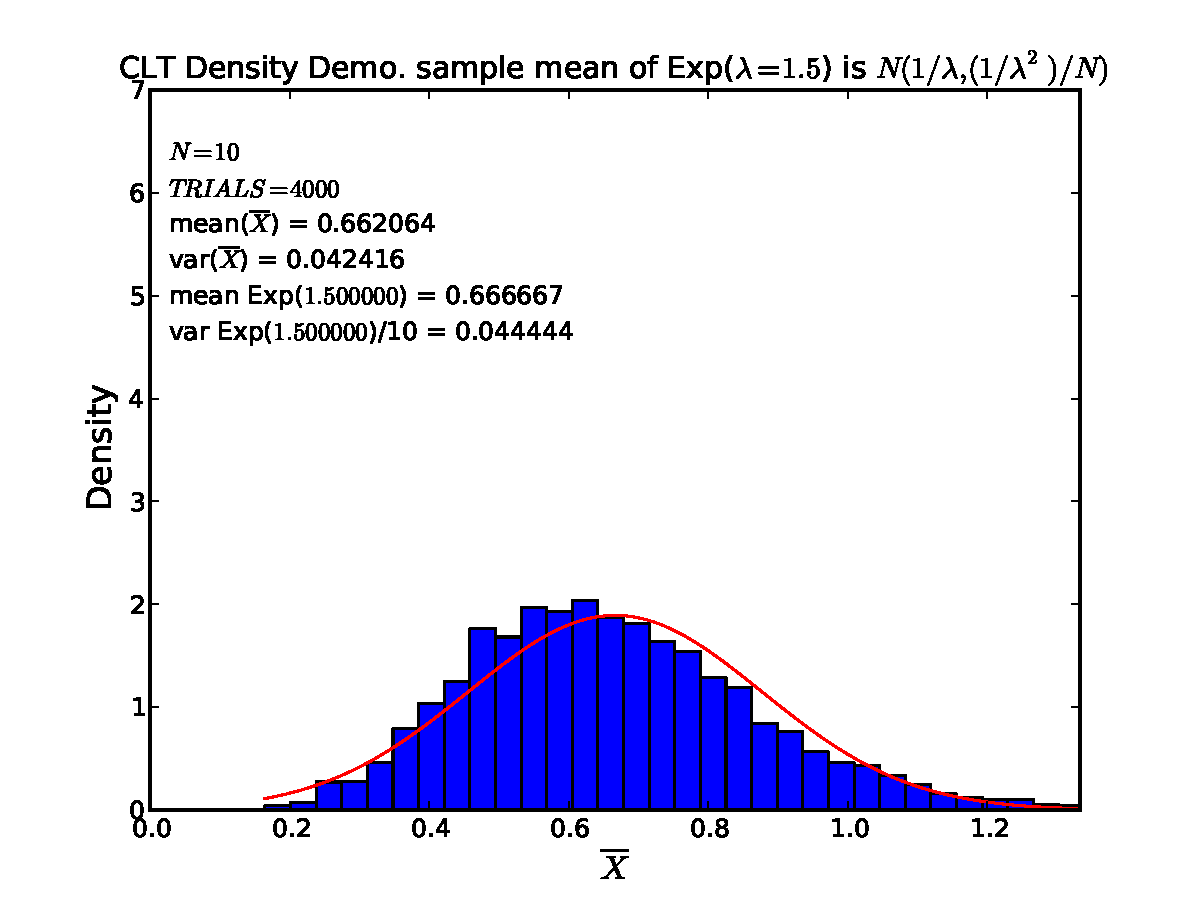
\includegraphics{figures/clt_exp-4000-10.pdf}} \scalebox{.33}{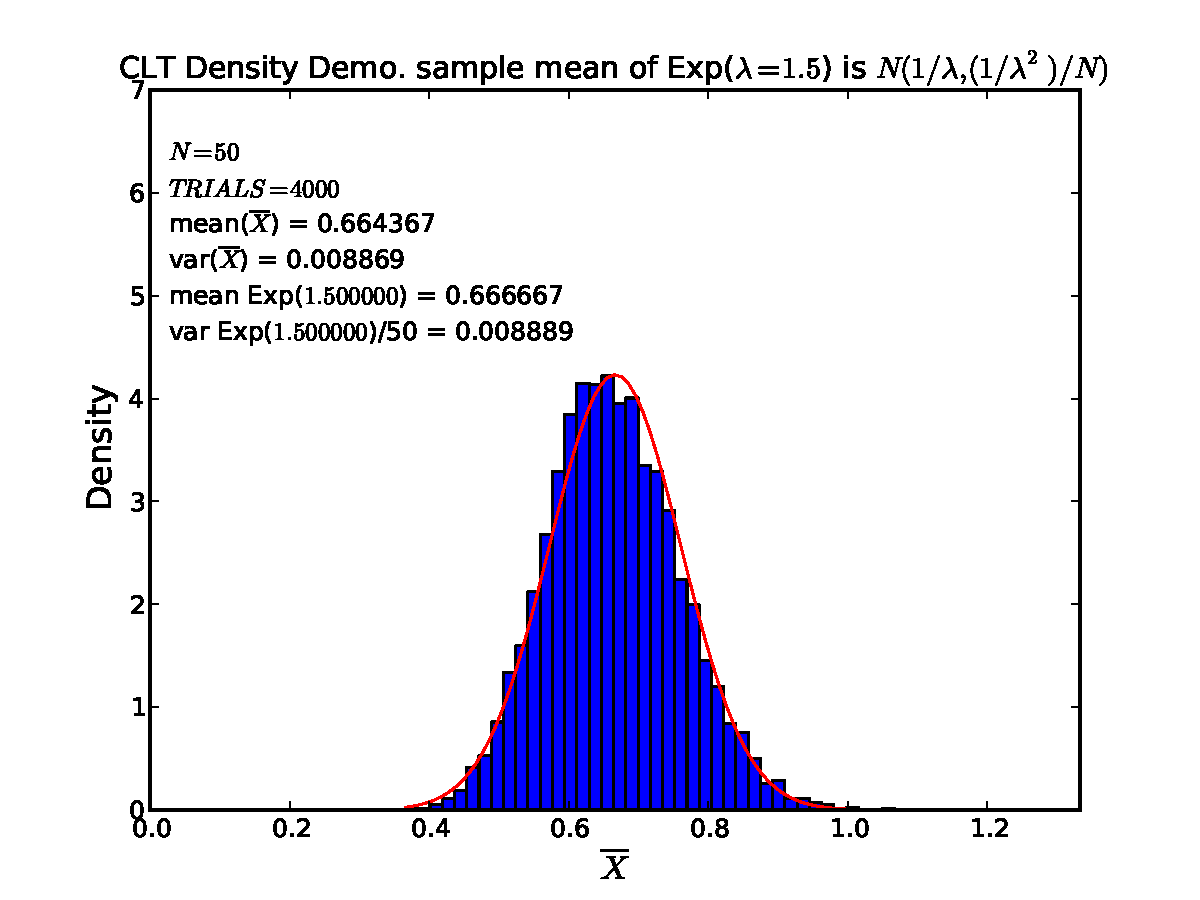
\includegraphics{figures/clt_exp-4000-50.pdf}}

Notice that there is a slight leftward bias in that the normal distribution is a little bit to the right it looks like. This is to be expected. You really need to bump up $N$ before you see it converge to the proper alignment.\\

\step Play around with other values of lambda and N.

\section{Deliverables}

Please submit:

\begin{itemize}
\item both {\tt clt\_unif.py}, {\tt clt\_exp.py} files
\item your {\tt varunif.py} used by your code
\item a PDF for $N=20$, $TRIALS=2000$ for CLT $U(0,1)$ demo
\item a PDF for $N=50$, $TRIALS=4000$, $\lambda=1.5$ for CLT $Exp(\lambda)$ demo
\end{itemize}

\end{fullwidth}
